\documentclass[10pt]{beamer}
\usetheme{Madrid}
\usepackage{amsmath,booktabs,hyperref}
\usepackage{tikz,graphicx}
\setbeamertemplate{navigation symbols}{}
\title{ZKP-Authorized Homomorphic Matching}
\subtitle{Auditable Record Revocation for Organ Donation\\Synthetic Research Prototype, Protocol v2}
\author{Chirag Parmar\\M250738CS}
\institute{NIT Calicut\\Guided by Dr. Abidha V.P. and Dr. Bijoy Das}
\date{October 2026}
\begin{document}
\begin{frame}\titlepage\end{frame}
\begin{frame}{Problem and scope}
\begin{itemize}
\item Approved stakeholder access to sensitive records and computations.
\item Confidential off-chain storage with auditable lifecycle metadata.
\item Recovery when the API or cleanup worker is unavailable.
\item Local development chain and synthetic data only.
\end{itemize}
\begin{block}{Trust boundary}The backend is trusted for encryption and result decryption. Browser ZKP generation protects the credential secret from the API. Wallet activity remains linkable.\end{block}
\end{frame}
\begin{frame}{Research questions}
\begin{enumerate}
\item Does approved membership enforce the intended role policy?
\item What overhead does ZKP authorization add to wallet RBAC?
\item Do BFV results equal the independent plaintext calculation?
\item Do encrypted records and revocation work survive downtime?
\end{enumerate}
\end{frame}
\begin{frame}{What changed after implementation review}
\begin{itemize}
\item Independent administrative enrollment replaces self-selected roles.
\item Authorization sessions replace the unsupported FE-key claim.
\item Opaque IDs/anchors replace plaintext clinical metadata on-chain.
\item Approved record-ID evaluation replaces arbitrary decryption.
\item Browser proving, persistent encrypted keys and durable cleanup.
\end{itemize}
\end{frame}
\begin{frame}{Prior work and positioning}
\begin{itemize}
\item Hawashin et al., IEEE Access 2022: private-Ethereum organ workflow.
\item Vanin et al., Sensors 23(1): blockchain/storage/HE healthcare integration.
\item Egala, Pradhan and Gupta: Block-Privacy combines blockchain, IPFS, ZK protocols and FE.
\item This work evaluates an explicitly trusted BFV implementation with approved membership and recoverable local revocation.
\end{itemize}
No new FE construction or ``first system'' claim. Unverified prior-work feature comparisons are excluded.
\end{frame}
\begin{frame}{Architecture and information exposure}
\begin{enumerate}
\item Browser: random credential, local proof worker, wallet transactions.
\item Administrator CLI: approved public leaves and membership-root publication.
\item Trusted API: signatures, authorization checks, BFV encryption/evaluation/decryption.
\item SQLite: public membership, encrypted keys, mappings and cleanup jobs.
\item Kubo: AES-wrapped BFV bundles; chain: opaque anchors and lifecycle events.
\end{enumerate}
Plaintext inputs are visible to the service during encryption. Chain metadata and prior released outputs remain visible.
\end{frame}
\begin{frame}{Protocol components and trust boundaries}
\begin{center}\begin{minipage}{.72\linewidth}
% Shared by the paper and presentation. Dashed boxes are trust domains.
\resizebox{\linewidth}{!}{%
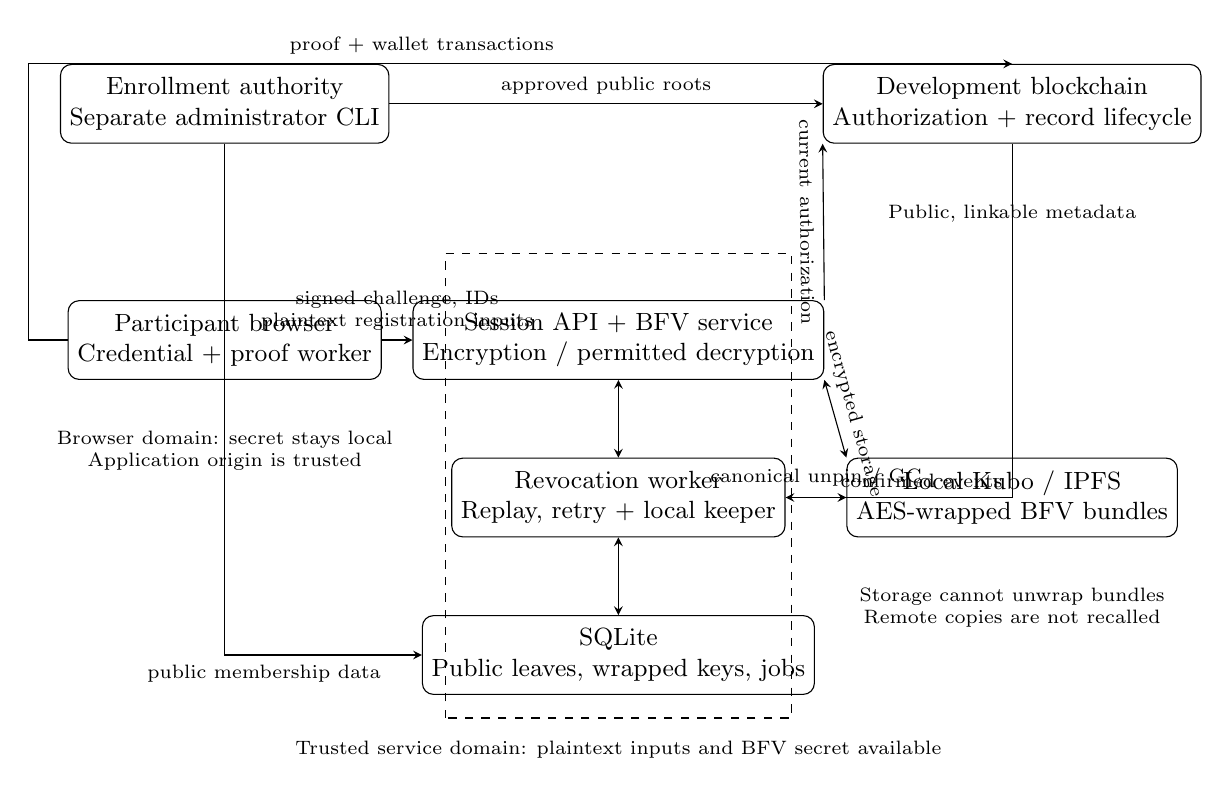
\begin{tikzpicture}[>=stealth,box/.style={draw,rounded corners,align=center,minimum width=3.3cm,minimum height=1cm,font=\small},every edge/.style={draw,->},every edge quotes/.style={font=\scriptsize}]
\node[box] (admin) at (-5,3) {Enrollment authority\\Separate administrator CLI};
\node[box] (browser) at (-5,0) {Participant browser\\Credential + proof worker};
\node[box] (chain) at (5,3) {Development blockchain\\Authorization + record lifecycle};
\node[box] (api) at (0,0) {Session API + BFV service\\Encryption / permitted decryption};
\node[box] (worker) at (0,-2) {Revocation worker\\Replay, retry + local keeper};
\node[box] (db) at (0,-4) {SQLite\\Public leaves, wrapped keys, jobs};
\node[box] (ipfs) at (5,-2) {Local Kubo / IPFS\\AES-wrapped BFV bundles};
\draw[dashed] (-2.2,-4.8) rectangle (2.2,1.1);
\node[font=\scriptsize,align=center] at (0,-5.2) {Trusted service domain: plaintext inputs and BFV secret available};
\draw[->] (admin) -- node[above,font=\scriptsize] {approved public roots} (chain);
\draw[->] (browser) -- node[above,font=\scriptsize,align=center] {signed challenge, IDs\\plaintext registration inputs} (api);
\draw[->] (browser.west) -- ++(-.5,0) |- node[pos=.7,above,font=\scriptsize] {proof + wallet transactions} (chain.north);
\draw[->] (api.north east) -- node[below,font=\scriptsize,sloped] {current authorization} (chain.south west);
\draw[->] (chain.south) |- node[pos=.7,above,font=\scriptsize] {confirmed events} (worker.east);
\draw[<->] (api) -- (worker);
\draw[<->] (worker) -- (db);
\draw[<->] (api.south east) -- node[above,font=\scriptsize,sloped] {encrypted storage} (ipfs.north west);
\draw[->] (worker) -- node[above,font=\scriptsize] {canonical unpin / GC} (ipfs);
\draw[->] (admin.south) |- node[pos=.6,below,font=\scriptsize] {public membership data} (db.west);
\node[font=\scriptsize,align=center] at (-5,-1.4) {Browser domain: secret stays local\\Application origin is trusted};
\node[font=\scriptsize,align=center] at (5,1.6) {Public, linkable metadata};
\node[font=\scriptsize,align=center] at (5,-3.4) {Storage cannot unwrap bundles\\Remote copies are not recalled};
\end{tikzpicture}%
}

\end{minipage}\end{center}
\end{frame}
\begin{frame}{Enrollment and proof binding}
\[
L=H(s,r),\quad r\in\{0,\ldots,5\}
\]
\begin{itemize}
\item Institution approves the public leaf; login never modifies the tree.
\item Depth-20 membership path with boolean selectors.
\item Public proof inputs bind recipient, chain, issuer and root version.
\item Nullifier prevents reuse of a submitted proof.
\item Root changes invalidate older sessions; keys/credentials are distinct.
\end{itemize}
\end{frame}
\begin{frame}{Authorized API and roles}
\small
\begin{tabular}{lcccc}\toprule
Role & Donor & Recipient & Match & Revoke\\\midrule
Doctor & Yes & Yes & Yes & No\\
Coordinator & Yes & Yes & Yes & No\\
Procurement & Yes & No & Yes & No\\
Matching & No & No & Yes & No\\
Transporter & No & No & No & No\\
Surgeon & No & No & Yes & Yes\\\bottomrule
\end{tabular}
\vspace{1em}
\begin{itemize}
\item Five-minute single-use signed challenge; four-hour maximum authorization.
\item Every protected operation checks current role, version and expiry.
\item Matching accepts canonical record IDs, never arbitrary ciphertexts.
\end{itemize}
\end{frame}
\begin{frame}{Encrypted records and restart recovery}
\begin{itemize}
\item Nine BFV ciphertexts: two ABO flags, six synthetic feature bits, urgency.
\item Each record bundle gets a separate AES-GCM wrapping key.
\item BFV secret and record keys are encrypted at rest under an operator secret.
\item Missing/wrong keys fail explicitly; no silent key replacement.
\item Only opaque identifiers, encrypted-content anchors and metadata go on-chain.
\end{itemize}
\end{frame}
\begin{frame}{Synthetic matching: eligibility before ranking}
\[
I=A_D(1-A_R)+B_D(1-B_R)
\]
Only $I=0$ is eligible; Rh and transplant exceptions are outside scope.
\[
m=\sum_{k=1}^{6}(d_k-r_k)^2,\quad u\in\{0,1,2\}
\]
\[
N=4200-700m+900u,\qquad S=\operatorname{round}(N/6)
\]
Experimental weights; toy markers are not clinical HLA typing. Ineligible pairs get no score. Eligible outputs are ranking points, not probabilities or organ allocations.
\end{frame}
\begin{frame}{Auditable local revocation}
\begin{itemize}
\item Surgeon deactivates donor or recipient by canonical opaque ID.
\item Deactivation blocks evaluation before cleanup completes.
\item Worker catches up missed logs, deletes the service-held record key, unpins and runs local GC.
\item Errors remain visible and retry with backoff.
\item Bounded keeper processing supports scheduled retention.
\end{itemize}
Local cleanup cannot erase external replicas, copied keys, backups or previously learned outputs. No universal-erasure or GDPR-compliance claim.
\end{frame}
\begin{frame}{Validation and experimental method}
\begin{itemize}
\item Real Groth16 proofs: two members, public-signal tampering and wrong sender.
\item HTTP tests: signatures, replay, permissions, expiry and batch ownership.
\item BFV: ABO pairs, feature boundaries, urgency and seeded cases.
\item Recovery: encrypted keys, missed events and failed-cleanup retries.
\item Live browser, isolated Kubo and local EVM acceptance demonstration.
\end{itemize}
Enabled full run: 28 passing tests, zero skips; 11 live checks. Browser tests use an EIP-1193 development-wallet adapter; manual MetaMask extension validation remains separate.
\end{frame}
\begin{frame}{Performance evaluation}
\begin{itemize}
\item Ten warmups and thirty samples for every repeated timing metric.
\item Plaintext wallet RBAC, BFV wallet RBAC and BFV ZKP authorization.
\item Authenticated HTTP jobs: $1\times1$, $5\times5$, $10\times10$.
\item Raw samples, median, p95, hardware, source/artifact hashes retained.
\item Proof time, verification gas, storage, evaluation and release separated.
\item Local receipts and direct cleanup timed separately; initial issuance gas recorded separately.
\end{itemize}
\IfFileExists{results-slides-v2.tex}{\small Measured local medians: Node proving 2922.3 ms; BFV evaluation 230.7 ms; verification and authorization 310,463 gas.
}{Numerical results are provisional until the revised benchmark finishes. Historical prototype timings are not reused.}
\end{frame}
\begin{frame}{Limitations and future work}
\begin{itemize}
\item Centralized decryption and linkable metadata remain explicit assumptions.
\item Synthetic scoring is not clinically validated.
\item Single-contributor development setup and local-chain measurements.
\item Production governance, key custody, dependency remediation and clinical review remain.
\item Actual FE, post-quantum components and multi-hospital deployment require separate research.
\end{itemize}
\end{frame}
\begin{frame}{Conclusion}
The revised system demonstrates approved ZKP membership, fixed BFV computation, encrypted records and recoverable local revocation under stated assumptions.
\vspace{1em}
Its contribution is a testable protocol integration and reproducible evaluation, not a new primitive or a clinical allocation system.
\end{frame}
\end{document}
